%===================================================================================================
\section{Motivation}{}
%---------------------------------------------------------------------------------------------------
\begin{frame}{HIV Epidemic: Context}
  \parpause{Eswatini:}
  \vhskip{-.5}{.67}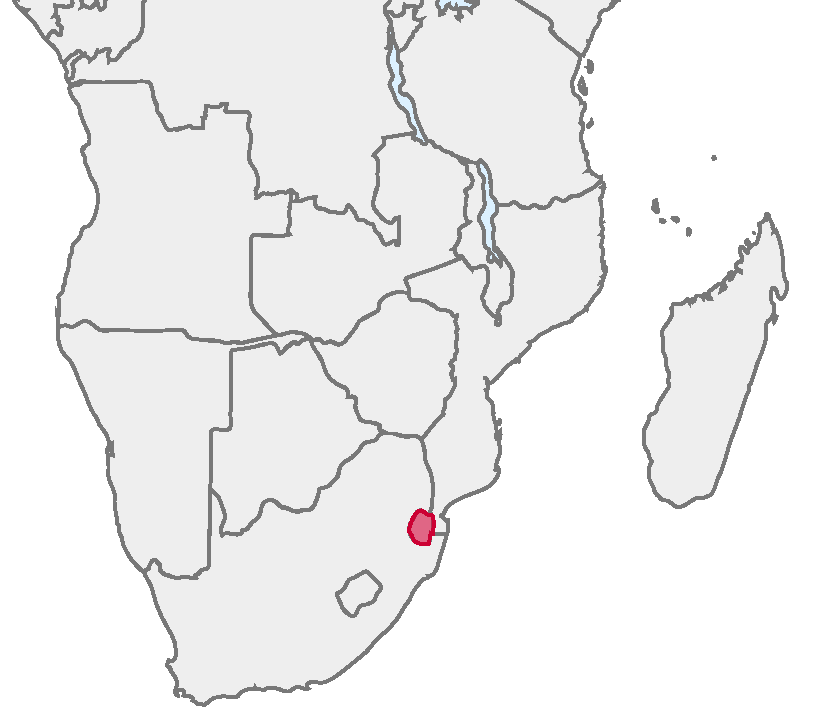
\includegraphics[height=6\baselineskip]{eswatini}\vhskip{-6.5}{0}
  \begin{itemize}
    \item Highest national HIV prevalence: 28\%
    \item Recently achieved 95-95-95 treatment cascade
  \end{itemize}
  \parpause{Key Populations, e.g. Female Sex Workers:}
  \begin{itemize}
    \item Disproportionate risk: acquisition + transmission
    \item Unique barriers to care
  \end{itemize}
\end{frame}
%---------------------------------------------------------------------------------------------------
\begin{frame}{HIV Epidemic: Transmission Modelling}
  \parpause{Applications:} \emph{mechanistic} insights, prediction, uncertainty analysis, \dots
  \parpause{Compartmental Models:} memoryless homogeneous groups
  \vhskip{-1}{.85}
\includegraphics[height=8\baselineskip]{model.si.inst.pdf}\vhskip{-8}{0}
  \parpause{Risk Heterogeneity:} acquisition, transmission, + interventions
  \begin{itemize}
    \item prior work: influences model outputs
    \item defined by: structure, data, equations \rarr \emph{assumptions}
  \end{itemize}
  \parpause{Overall Research Question:}\pars\rqstyle
  How do modelling assumptions influence outputs from HIV transmission models?
\end{frame}
%---------------------------------------------------------------------------------------------------
\begin{frame}{Overview}
  \paragraph{Chapter Research Questions:}
  In compartmental models of HIV transmission \dots\medskip\pause
  \begin{enumerate}[<+->]\setcounter{enumi}{1}\rqstyle
    \item[2.] How might \textbf{model assumptions} influence prevention impacts of treatment?
    \item[5.] How might \textbf{treatment coverage assumptions} influence prevention impacts?
    \item[3.] How can we improve assumptions in \textbf{model design \& parameterization}?
    \item[4.] How can we improve assumptions in \textbf{incidence equations}?
  \end{enumerate}
  \vfill
\end{frame}
%===================================================================================================
\section[2]{Scoping Review: Heterogeneity in Models}
  {How might model assumptions influence prevention impacts of treatment?}
%---------------------------------------------------------------------------------------------------
\newcommand{\itemdir}[1]{\item[$\boldsymbol{#1}$]}
\begin{frame}{Scoping Review: Missing Heterogeneity}
  \parbox{.5\textwidth}{\pause%
    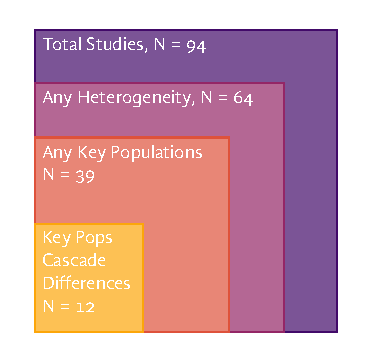
\includegraphics[width=.5\textwidth]{api.blocks}}%
  \parbox{.5\textwidth}{
    \parpause{Prevention impacts of treatment:}\pause%
    \begin{itemize}[<+->]
      \itemdir{\sim} Risk heterogeneity
      \itemdir{\downarrow} Risk heterogeneity + turnover
      \itemdir{\uparrow} KP cascade prioritized
      \itemdir{?\downarrow} KP cascade lagging
    \end{itemize}}
\end{frame}
%===================================================================================================
\section[5]{Intersecting Risk \& Treatment Gaps}
  {How might treatment coverage assumptions influence treatment impacts?}
%---------------------------------------------------------------------------------------------------
\begin{frame}{Treatment as Prevention: Impact of Who is Left Behind}
  \vhskip{0}{.1}\pause\textbf{Observed} 95-95-95: base case\enspace\emph{vs}\dots
  \vhskip{0}{.1}\pause\textbf{Hypothetical} 80-80-90: groups left behind
  \parpause{}
  \centering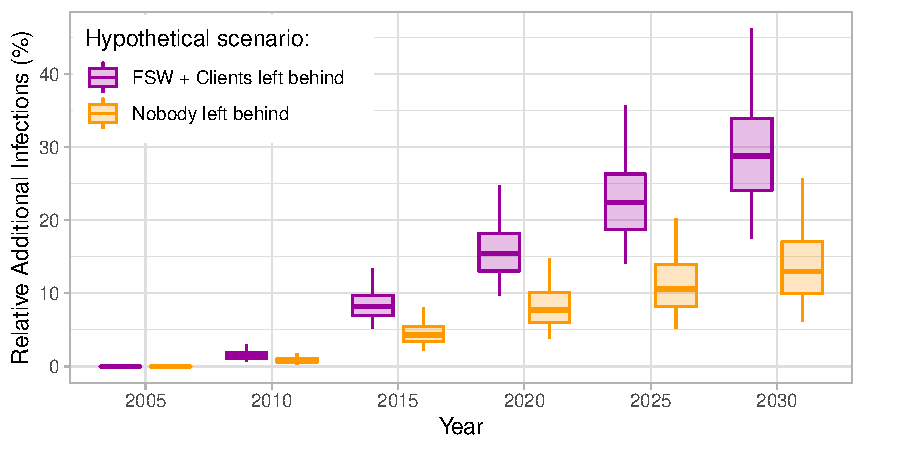
\includegraphics[width=.8\textwidth]{art.1.rai.simple.e}
\end{frame}
%===================================================================================================
\section[3]{Model Design, Parameterization, \& Calibration}
  {How can we improve assumptions in model design \& parameterization?}
%---------------------------------------------------------------------------------------------------
\newcommand{\method}[2]{\pause\parbox{.45\textwidth}{#1}\pause\rarr\enspace{#2}}
\begin{frame}{Model Design \& Parameterization: Usual Assumptions}
  \begin{enumerate}
    \item[]\textbf{\method{Usual Assumption}{Data-Informed Assumption}}\medskip
    \item\method{No main partnerships between KP}{overlapping partnership types}
    \item\method{KP are homogeneous}{higher vs lower risk FSW + clients}
    \item\method{Reported partners unbiased}{adjust using polling-booth data}
    \item\method{Reported partners = rate}{adjust for partnership duration}
    \item\method{1 degree of freedom mixing}{flexible log-linear mixing}
    \item\method{No risk group turnover}{turnover framework}
  \end{enumerate}
\end{frame}
%---------------------------------------------------------------------------------------------------
\begin{frame}{Model Design \& Parameterization: Eswatini Model}
  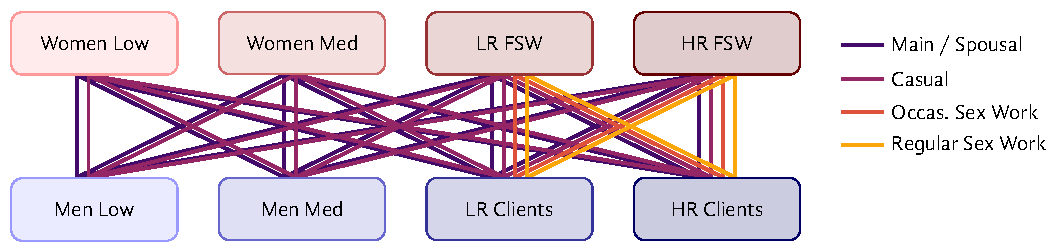
\includegraphics[scale=.6]{model.risk}\par\pause
  \medskip
  \begin{itemize}[<+->]
    \item[] Eswatini data sources:
    \item Household surveys: '06, '11, '16
    \item FSW surveys: '11, '14, '21
  \end{itemize}
\end{frame}
%===================================================================================================
\section[4]{Effective Partnerships Adjustment}
  {How can we improve assumptions in incidence equations?}
%---------------------------------------------------------------------------------------------------
\begin{frame}{Usual Assumption: Instantaneous Partnerships}
  \parpause{Why:} memoryless homogeneous compartments\\
  \hphantom{\textbf{Why:}} \emph{cannot} track individual partnerships
  \vhskip{-2}{.7}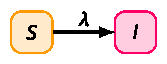
\includegraphics[height=2\baselineskip]{model.si.inst.hor}\vhskip{-1}{0}
  \parpause{How:} model partnerships as a \emph{rate}, with cumulative risk \emph{per-partnership}
  \parpause{But:} adjusting for ``\textcolor{tx}{wasted sex acts}'':\medskip\pause\par
  \begin{itemize}[<+->]
    \item \emph{within} partnerships
    \item \emph{between} partnerships
  \end{itemize}
  \vhskip{-4}{.4}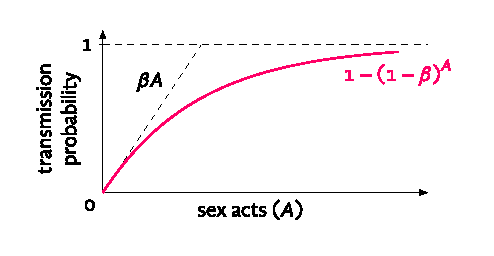
\includegraphics[scale=.8]{binom.dur.e1}
\end{frame}
%---------------------------------------------------------------------------------------------------
\newcommand{\tradeoff}[3]{\parbox[b]{16mm}{\strut#2} \rarr \coloremph{#1}{#3} wasted acts}
\begin{frame}{Instantaneous Partnerships: Problems}
  \pause
  \begin{enumerate}[<+->]
    \item \textbf{Instant risk} of onward transmission
    \item Wasted sex acts \emph{within} partnerships
          \\\rarr \textbf{trade off}:\par
    \vhskip{-2}{.5}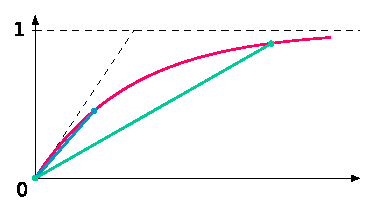
\includegraphics[scale=.8]{binom.dur.e2}\vhskip{-4.5}{0}
    \begin{itemize}
      \item \tradeoff{rd}{full duration}{frontload}
      \item \tradeoff{ry}{1-year only}{ignore}
    \end{itemize}
    \item Wasted sex acts \coloremph{py}{between} partnerships
          \\\rarr \textbf{unnecessary}
    % \item Within vs between partnership heterogeneity \dots
  \end{enumerate}
\end{frame}
%---------------------------------------------------------------------------------------------------
\begin{frame}{Effective Partnerships Adjustment}
  \parpause{Core Idea:} People who recently \emph{acquired or transmitted}
    \rarr \coloremph{tx!50}{holding state}
  \par\hphantom{\textbf{Core Idea:}~}(remove from incidence equation)
  \parpause{Details:}\pause
  \begin{itemize}[<+->]
    \item Remove until: partnerships change $\delta^{-1}$
    \item If 2+ partnerships: decrease partners by 1
  \end{itemize}
  \vhskip{-4}{.67}\parbox[t]{.33\textwidth}{%
    \begin{tabular}{cc}
      Instant & Proposed \\
      
\includegraphics[scale=.8]{model.si.inst.pdf} &
      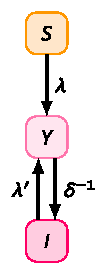
\includegraphics[scale=.8]{model.si.prop.pdf}
    \end{tabular}}\vhskip{-3}{}
\end{frame}
%---------------------------------------------------------------------------------------------------
\begin{frame}{Comparing Incidence Approaches: Equal Parameters}
  \foreach \i in {1,2,3,4}{\only<\i>{\includegraphics[width=\textwidth]{foi.ep.incidence.\i.pdf}}}
\end{frame}
%---------------------------------------------------------------------------------------------------
\begin{frame}{Comparing Incidence Approaches: Re-Fit Parameters}
  \foreach \i in {1,2,3,4}{\only<\i>{\includegraphics[width=\textwidth]{foi.tpaf.\i.pdf}}}
\end{frame}
%===================================================================================================
\section{Conclusion}{}
%---------------------------------------------------------------------------------------------------
\begin{frame}{Current Models Undervalue Key Populations}
  \pause
  \begin{enumerate}[<+->]
    \item \textbf{KP Not Modelled}
    \item \textbf{KP Simplified:} no turnover, no main partners, homogeneous
    \item \textbf{Incidence Equations:}
    \begin{itemize}
      \item 1-Year: too few wasted acts in \emph{long partnerships}
      \item Between-partnerships: too many wasted acts among \emph{higher risk}
    \end{itemize}
    \item \textbf{Assume Equal Interventions:} who is being left behind?
    \bigskip
    \item[\rarr]\textbf{Thesis:} + methods to improve these assumptions
  \end{enumerate}
\end{frame}
%---------------------------------------------------------------------------------------------------
\newcommand{\thankscol}[1]{\parbox[t]{.33333\textwidth}{\vskip-\baselineskip#1}\ignorespaces}
\newcommand{\thankshead}[1]{\vskip.5\baselineskip\textbf{#1}}
\newcommand{\thankslogo}[3][0]{\vhskip{.5}{#1}\includegraphics[height=#2\baselineskip]{#3}}
\begin{frame}{Thanks}\fontsize{8pt}{9pt}\selectfont
  \thankscol{
    \thankshead{Supervisor}
    \\Sharmistha Mishra
    \thankshead{Thesis Committee}
    \\Michael Escobar
    \\Rupert Kaul
    \thankshead{Internal Team}
    \\Kristy Yiu
    \\Huiting Ma
    \\Linwei Wang
    \\Ekta Mishra
    \\Korryn Bodner
    \\Alex Whitlock
    \\Siyi Wang
    \\Oliver Gatalo
    \\Suzanne Shoush
    \\Mackenzie Hamilton
    \\Samantha Lo}
  \thankscol{
    \thankshead{Examiners}
    \\Leigh Johnson
    \\Ashleigh Tuite
    \\Nicole Mideo
    \\Marie Claude Boily
    \thankshead{External Collaborators}
    \\Stefan Baral
    \\Sheree Schwartz
    \\Amrita Rao
    \\Bheki Sithole
    \\Sindy Matse
    \\Laura Muzart
    \\Zandile Mnisi
    \thankshead{Survey Respondents}
    \thankshead{Service Providers}
    \thankshead{\rlap{R, Python, \LaTeX, Linux, Communities}}}
  \thankscol{
    \thankshead{Funding \& Support}
    \thankslogo[.00]{1.2}{map}
    \thankslogo[.00]{1.3}{smh}
    \thankslogo[.00]{2.2}{uoft}
    \thankslogo[.00]{1.8}{nserc}
    \thankslogo[.00]{1.5}{on}\vskip.5\baselineskip
    \thankslogo[.00]{1.7}{drac}
    \thankshead{Ali, Friends \& Family}}
\end{frame}
% ===================================================================================================